\documentclass[11pt,a4paper]{article}
\usepackage[utf8]{inputenc}
\usepackage[T1]{fontenc}
\usepackage{lmodern}
\usepackage[margin=2.5cm]{geometry}
\usepackage{booktabs}
\usepackage{graphicx}
\usepackage{caption}
\usepackage{float}
\usepackage{amsmath}
\usepackage{breqn}
\usepackage[hidelinks]{hyperref}

\title{An automatic report for the dataset: 07-call-centre}
\author{Some Math empowered by some AI guided by some researchers}
\date{10 November 2026}

\begin{document}
\maketitle

\noindent\emph{Produced by \texttt{autostat}, a Python 3 port of the Automatic Bayesian Covariance Discovery system of Lloyd et al. (AAAI 2014).}


\begin{figure}[H]
\centering
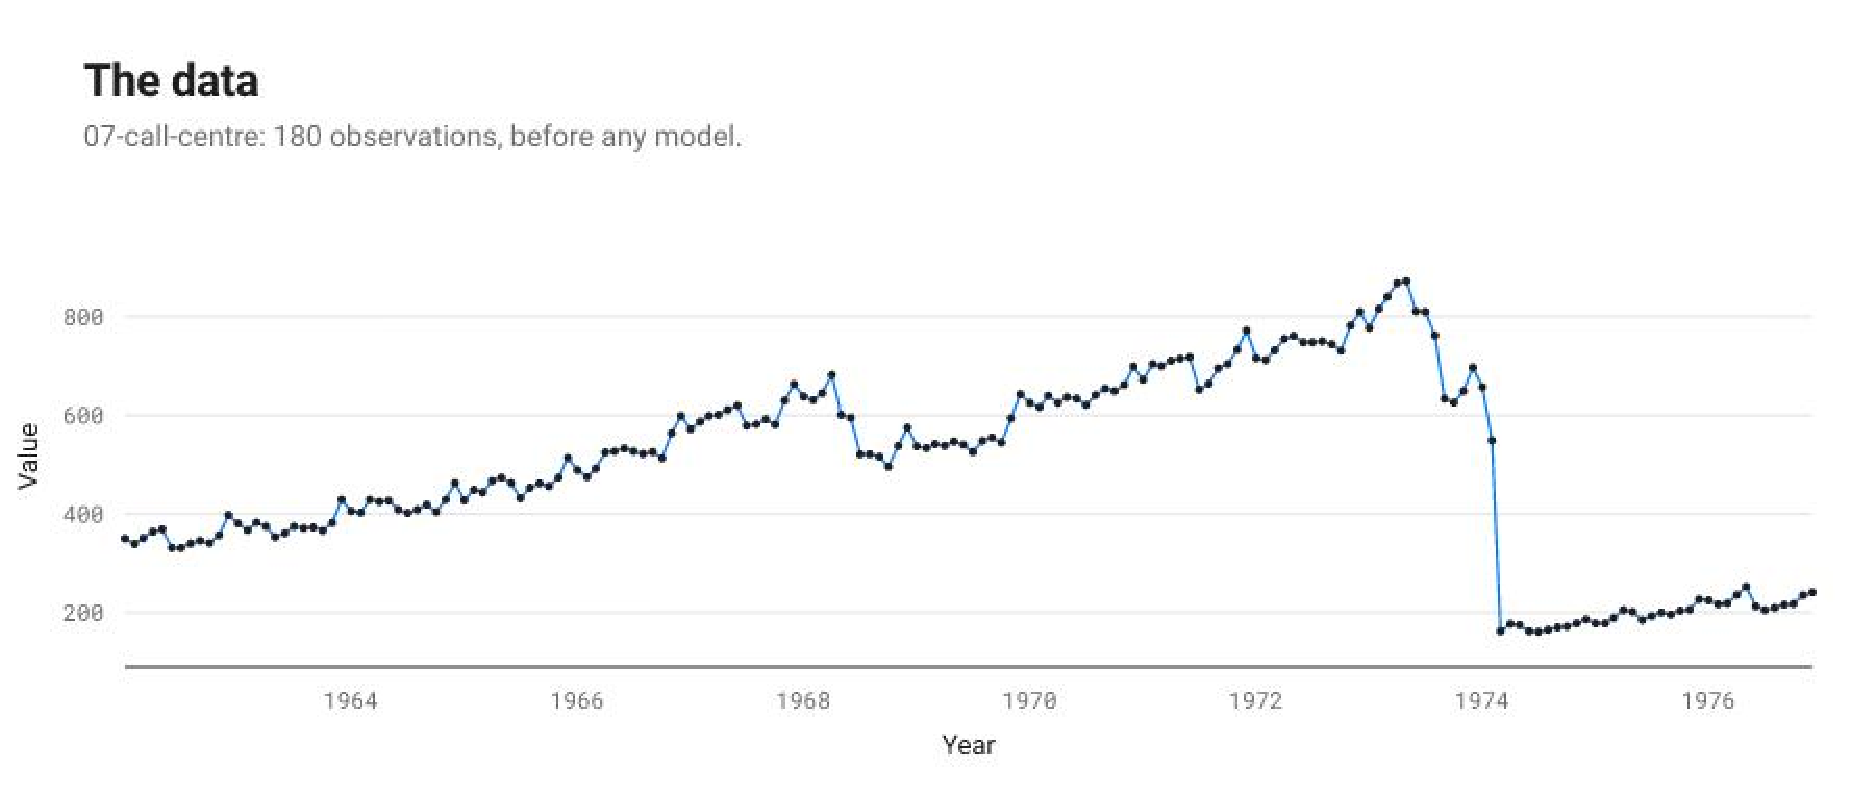
\includegraphics[width=\linewidth]{data.pdf}
\caption*{The data}
\end{figure}

\section*{Executive summary}

The structure search selected \texttt{CP(Lin + Per + Lin x SE, SE) + CW(WN, WN)} (Bayesian information criterion 1631.6; negative log likelihood 771.7 on 180 points). It decomposes into 6 additive components, listed by how much each reduces extrapolation error:
\begin{enumerate}
  \item A linearly increasing function. This function applies until Feb 1974.
  \item A very smooth monotonically increasing function. This function applies from Feb 1974 onwards.
  \item A smooth function with marginal standard deviation increasing linearly away from Feb 1964. This function applies until Feb 1974.
  \item A periodic function with a period of 1.0 years. This function applies until Feb 1974.
  \item Uncorrelated noise. This function applies until May 1973 and from Oct 1973 onwards.
  \item Uncorrelated noise. This function applies from May 1973 until Oct 1973.
\end{enumerate}

\begin{center}
\begin{tabular}{lrrrr}
\toprule
\# & $R^2$ cumulative (\%) & Residual variance explained (\%) & CV MAE & MAE reduction (\%) \\
\midrule
data & & & 492 & \\
1 & 77.5 & 77.5 & 66.3 & 86.5 \\
2 & 94.5 & 75.4 & 31.9 & 51.9 \\
3 & 99.1 & 84.0 & 24.2 & 24.1 \\
4 & 99.7 & 66.6 & 21 & 13.4 \\
5 & 99.9 & 74.0 & 21 & 0.0 \\
6 & 100.0 & 100.0 & 21 & 0.0 \\
\bottomrule
\end{tabular}
\end{center}

MAE: mean absolute error over ten contiguous held-out blocks; CV: cross-validated.

\section*{The formula found}

The structure search is a symbolic regression: it searches a grammar of expressions over kernels and keeps the one with the lowest Bayesian information criterion. This is the expression it kept, with every fitted parameter in place; $t$ is in years.
\begin{dmath*}
y(t) = f_{1}(t) + f_{2}(t) + f_{3}(t) + f_{4}(t) + f_{5}(t) + f_{6}(t)
\end{dmath*}

Each component is a Gaussian process with its own covariance:
\begin{dmath*}
f_{1}(t) \sim \mathrm{GP}\!\left(0,\ (1 - w_{1}(t))(1 - w_{1}(t'))\left[1576\,(t - 1954)(t' - 1954)\right]\right)
\end{dmath*}
\begin{dmath*}
f_{2}(t) \sim \mathrm{GP}\!\left(0,\ w_{1}(t)\,w_{1}(t')\left[50972\,\exp\!\left(-\frac{(t - t')^2}{2 \cdot 8.54^2}\right)\right]\right)
\end{dmath*}
\begin{dmath*}
f_{3}(t) \sim \mathrm{GP}\!\left(0,\ (1 - w_{1}(t))(1 - w_{1}(t'))\left[81.95\,(t - 1964)(t' - 1964) \cdot \exp\!\left(-\frac{(t - t')^2}{2 \cdot 0.2951^2}\right)\right]\right)
\end{dmath*}
\begin{dmath*}
f_{4}(t) \sim \mathrm{GP}\!\left(0,\ (1 - w_{1}(t))(1 - w_{1}(t'))\left[264.9\,\frac{\exp\!\left(4.487\cos\frac{2\pi (t - t')}{0.9981}\right) - I_0(4.487)}{e^{4.487} - I_0(4.487)}\right]\right)
\end{dmath*}
\begin{dmath*}
f_{5}(t) \sim \mathrm{GP}\!\left(0,\ (1 - w_{2}(t))(1 - w_{2}(t'))\left[109.5\,\delta_{t t'}\right]\right)
\end{dmath*}
\begin{dmath*}
f_{6}(t) \sim \mathrm{GP}\!\left(0,\ w_{2}(t)\,w_{2}(t')\left[993.7\,\delta_{t t'}\right]\right)
\end{dmath*}

The changes of regime weigh the components with:
\begin{dmath*}
w_{1}(t) = \tfrac{1}{2}\left(1 + \tanh\left(43.34\,(t - 1974)\right)\right)
\end{dmath*}
\begin{dmath*}
w_{2}(t) = \tfrac{1}{4}\left(1 + \tanh\left(18.01\,(t - 1973)\right)\right)\left(1 - \tanh\left(18.01\,(t - 1974)\right)\right)
\end{dmath*}

These components have a closed form, read from their posterior mean:
\begin{dmath*}
f_{1}(t) = (1 - w_{1}(t))\,\left(322.5 + 39.52\,(t - 1962)\right)
\end{dmath*}
\begin{dmath*}
f_{4}(t) \approx (1 - w_{1}(t))\,\left(14.51\cos\!\left(\frac{2\pi \cdot (t - 1962)}{0.9981} - 0.7209\right) + 9.851\cos\!\left(\frac{2\pi \cdot 2 \cdot (t - 1962)}{0.9981} + 1.462\right) + 10.23\cos\!\left(\frac{2\pi \cdot 3 \cdot (t - 1962)}{0.9981} + 1.178\right) + 8.749\cos\!\left(\frac{2\pi \cdot 4 \cdot (t - 1962)}{0.9981} + 2.129\right) + 2.103\cos\!\left(\frac{2\pi \cdot 5 \cdot (t - 1962)}{0.9981} + 2.963\right) + 1.802\cos\!\left(\frac{2\pi \cdot 6 \cdot (t - 1962)}{0.9981} + 2.254\right) + 0.2168\cos\!\left(\frac{2\pi \cdot 7 \cdot (t - 1962)}{0.9981} + 1.273\right) + 0.1321\cos\!\left(\frac{2\pi \cdot 8 \cdot (t - 1962)}{0.9981} + 2.168\right)\right)
\end{dmath*}

A periodic kernel is exactly a sum of cosines, so a periodic component is a Fourier series in its period; it is written up to the harmonic after which the rest weighs less than 0.1 % of the component, hence the approximate sign.

The other components are smooth, quasi-periodic or noise without a short formula: a draw from such a process has no finite closed form; its covariance above is the formula.

Closed form of each component:

\begin{center}\footnotesize
\begin{tabular}{lp{0.36\linewidth}l}
\toprule
\# & component & closed form \\
\midrule
1 & A linearly increasing function. This function applies until Feb 1974 & exact polynomial of degree 1 \\
2 & A very smooth monotonically increasing function. This function applies from Feb 1974 onwards & none: the covariance is the formula \\
3 & A smooth function with marginal standard deviation increasing linearly away from Feb 1964. This function applies until Feb 1974 & none: the covariance is the formula \\
4 & A periodic function with a period of 1.0 years. This function applies until Feb 1974 & Fourier series, 8 harmonics, largest gap 0.047 \% of the component \\
5 & Uncorrelated noise. This function applies until May 1973 and from Oct 1973 onwards & none: the covariance is the formula \\
6 & Uncorrelated noise. This function applies from May 1973 until Oct 1973 & none: the covariance is the formula \\
\bottomrule
\end{tabular}
\end{center}

\section*{Search path and stopping criterion}

The 2014 configuration searches a fixed number of levels and keeps the lowest BIC; it has no stopping rule. The table follows the winner of each level. A change of structure adds or removes terms; a level that keeps the structure only refits its parameters. BIC differences read on the scale of Kass and Raftery (1995): under 2 barely worth mentioning, 2 to 6 positive, 6 to 10 strong, over 10 very strong.

\begin{center}\footnotesize
\begin{tabular}{lllp{0.36\linewidth}lll}
\toprule
level & BIC & change & structure & components & closed & params \\
\midrule
1 & 1949.4 &  & SE + WN & 2 & 0 & 3 \\
2 & 1807.0 & -142.4 & CP(SE, SE) + WN & 3 & 0 & 7 \\
3 & 1717.1 & -89.9 & CP(Lin x SE + SE, SE) + WN & 4 & 0 & 10 \\
4 & 1696.7 & -20.4 & CP(Lin x SE + Per x SE + SE, SE) + WN & 5 & 0 & 14 \\
5 & 1659.7 & -37.0 & CP(Lin x SE + Per x SE + SE, SE) + WN & 5 & 0 & 14 \\
6 & 1648.1 & -11.6 & CP(Lin x SE + Per x SE + SE, SE) + WN & 5 & 0 & 14 \\
7 & 1641.1 & -7.0 & CP(Lin x SE + Per + SE, SE) + WN & 5 & 1 & 13 \\
8 & 1636.8 & -4.3 & CP(Lin + Lin x SE + Per, SE) + WN & 5 & 2 & 13 \\
9 & 1633.4 & -3.4 & CP(Lin + Lin x SE + Per, SE) + WN & 5 & 2 & 13 \\
10 (kept) & 1631.6 & -1.9 & CP(Lin + Lin x SE + Per, SE) + CW(WN, WN) & 6 & 2 & 17 \\
\bottomrule
\end{tabular}
\end{center}

\begin{figure}[H]
\centering
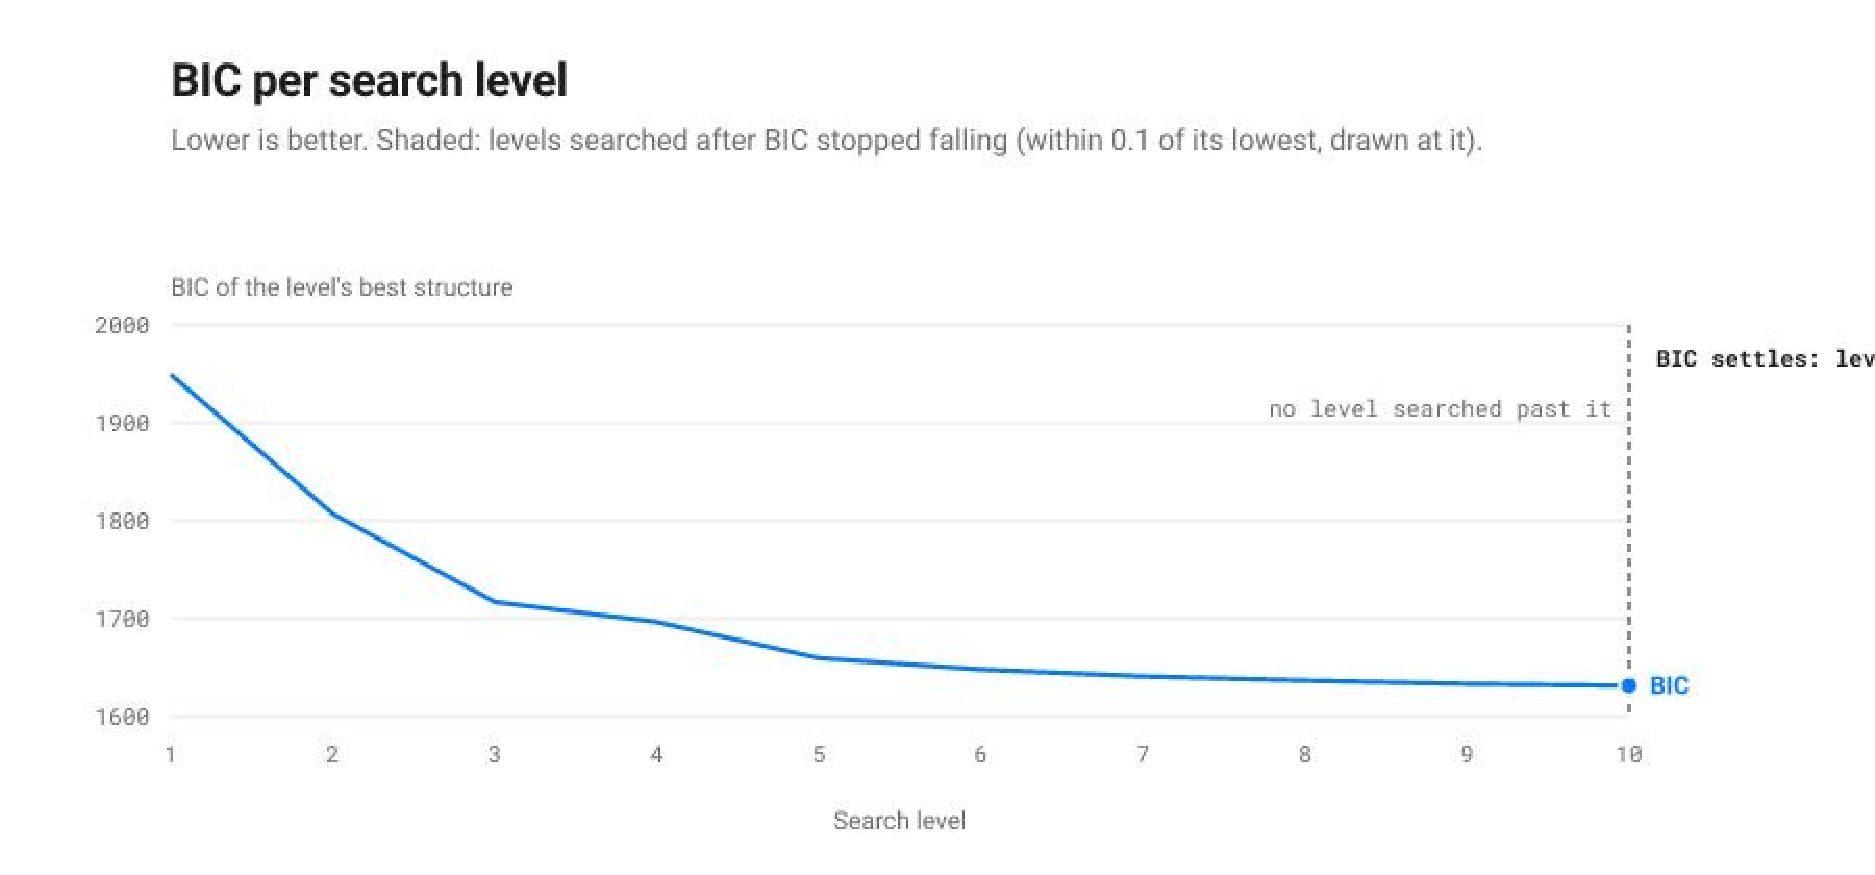
\includegraphics[width=\linewidth]{bic.pdf}
\caption*{BIC per search level}
\end{figure}

Posterior weight of each structure met, exp(-BIC/2) normalised under a flat prior, after the Bayesian machine scientist (Guimerà et al., 2020): where the search keeps one structure, the weights say how much the data prefer it to the others. The 4 structure(s) under 0.001 are left out.

\begin{center}\footnotesize
\begin{tabular}{p{0.36\linewidth}ll}
\toprule
structure & lowest BIC & weight \\
\midrule
CP(Lin + Lin x SE + Per, SE) + CW(WN, WN) & 1631.6 & 0.713 \\
CP(Lin + Lin x SE + Per, SE) + WN & 1633.4 & 0.281 \\
CP(Lin x SE + Per + SE, SE) + WN & 1641.1 & 0.006 \\
\bottomrule
\end{tabular}
\end{center}

\begin{itemize}
\item The search ran 10 levels (the published 2014 search: ten levels, no stopping rule) and keeps the model of level 10, CP(Lin + Lin x SE + Per, SE) + CW(WN, WN), BIC 1631.6.
\item The best different structure, CP(Lin + Lin x SE + Per, SE) + WN (level 9), is 1.9 above it: barely worth mentioning evidence for the kept one on the Kass and Raftery scale.
\item Weighed by exp(-BIC/2) under a flat prior, as the Bayesian machine scientist weighs expressions, the structures met give the kept one a posterior weight of 0.713 and the next, CP(Lin + Lin x SE + Per, SE) + WN, 0.281: the data barely tell them apart.
\item The last level still changed the structure and lowered BIC by 1.9: more levels might find a better expression.
\item A rule stopping after 1 level(s) without a fall above 0.1 would not have stopped within these 10 levels.
\item A rule stopping after 2 level(s) without a fall above 0.1 would not have stopped within these 10 levels.
\item The kept expression has 17 parameters for 180 points: its BIC is a fit term 2 NLL = 1543.3 plus a complexity term p ln n = 88.3, each extra parameter costing 5.19; it splits into 6 components, 2 of them with a closed form.
\end{itemize}

\begin{figure}[H]
\centering
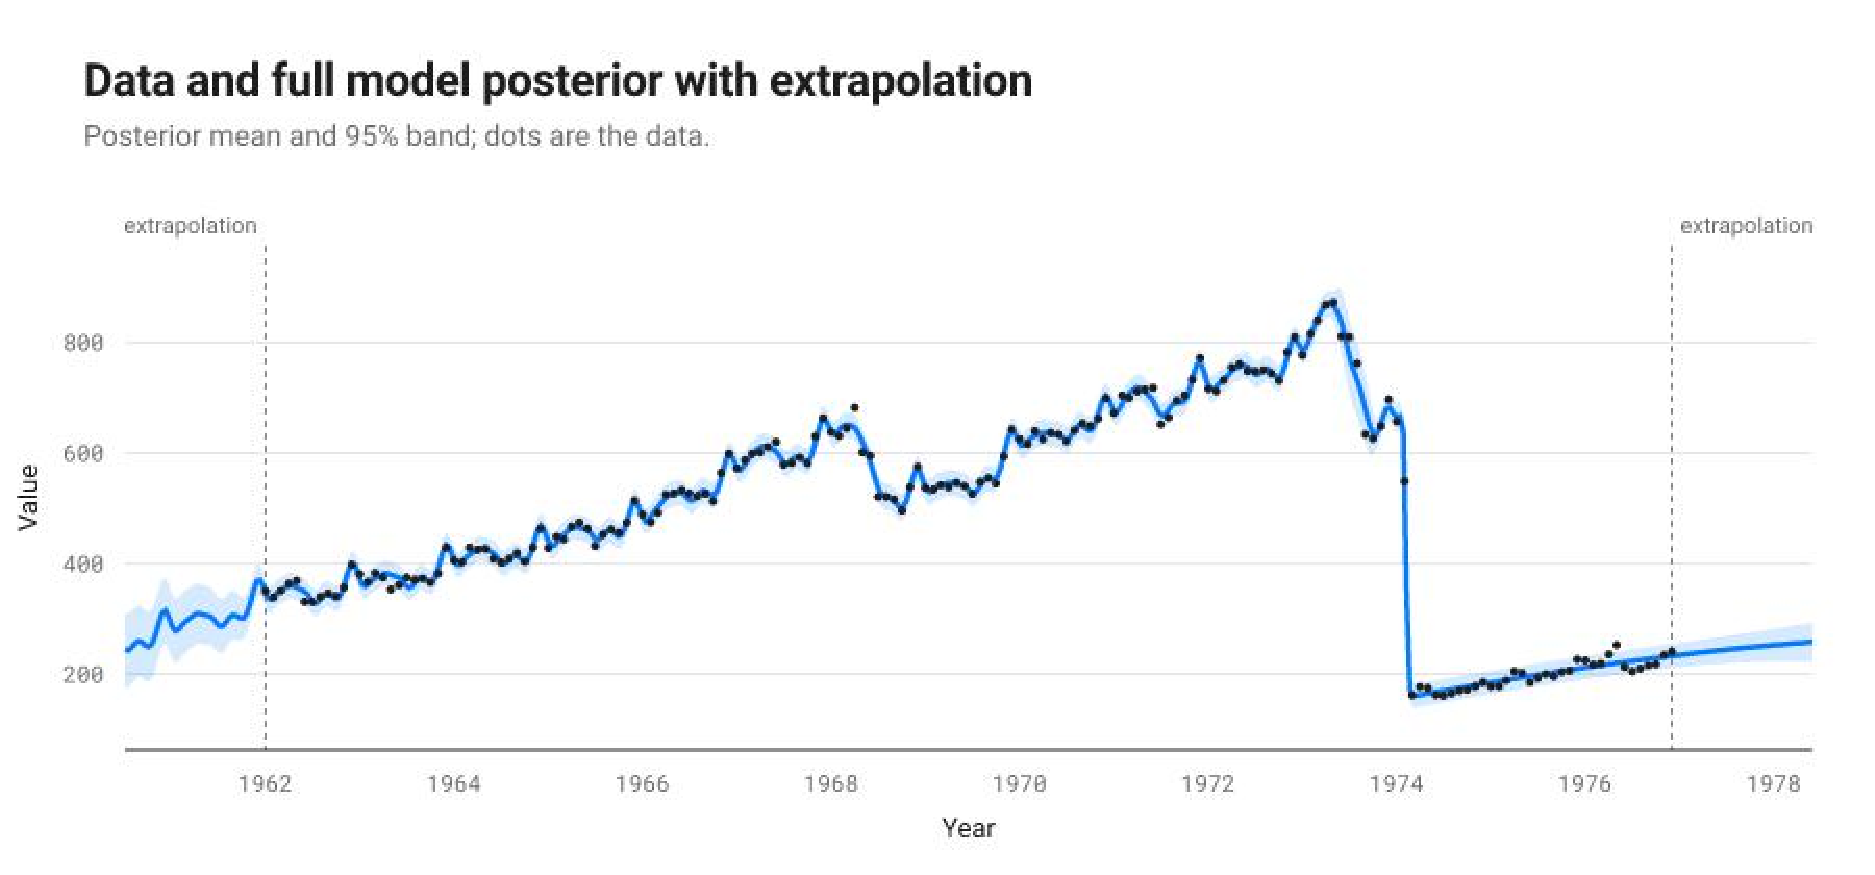
\includegraphics[width=\linewidth]{fit.pdf}
\caption*{Data and full posterior}
\end{figure}

\section*{Detailed discussion of the components}

\subsection*{Component 1: A linearly increasing function. This function applies until Feb 1974}

This component is linearly increasing. This component applies until Feb 1974.

This component explains 77.5\% of the data's variance on its own; with the components above it, 77.5\%. Adding it changes the cross-validated MAE by -86.5\%.

\emph{Extrapolation.} This component is assumed to stop before the end of the data and will therefore be extrapolated as zero.

\begin{figure}[H]
\centering
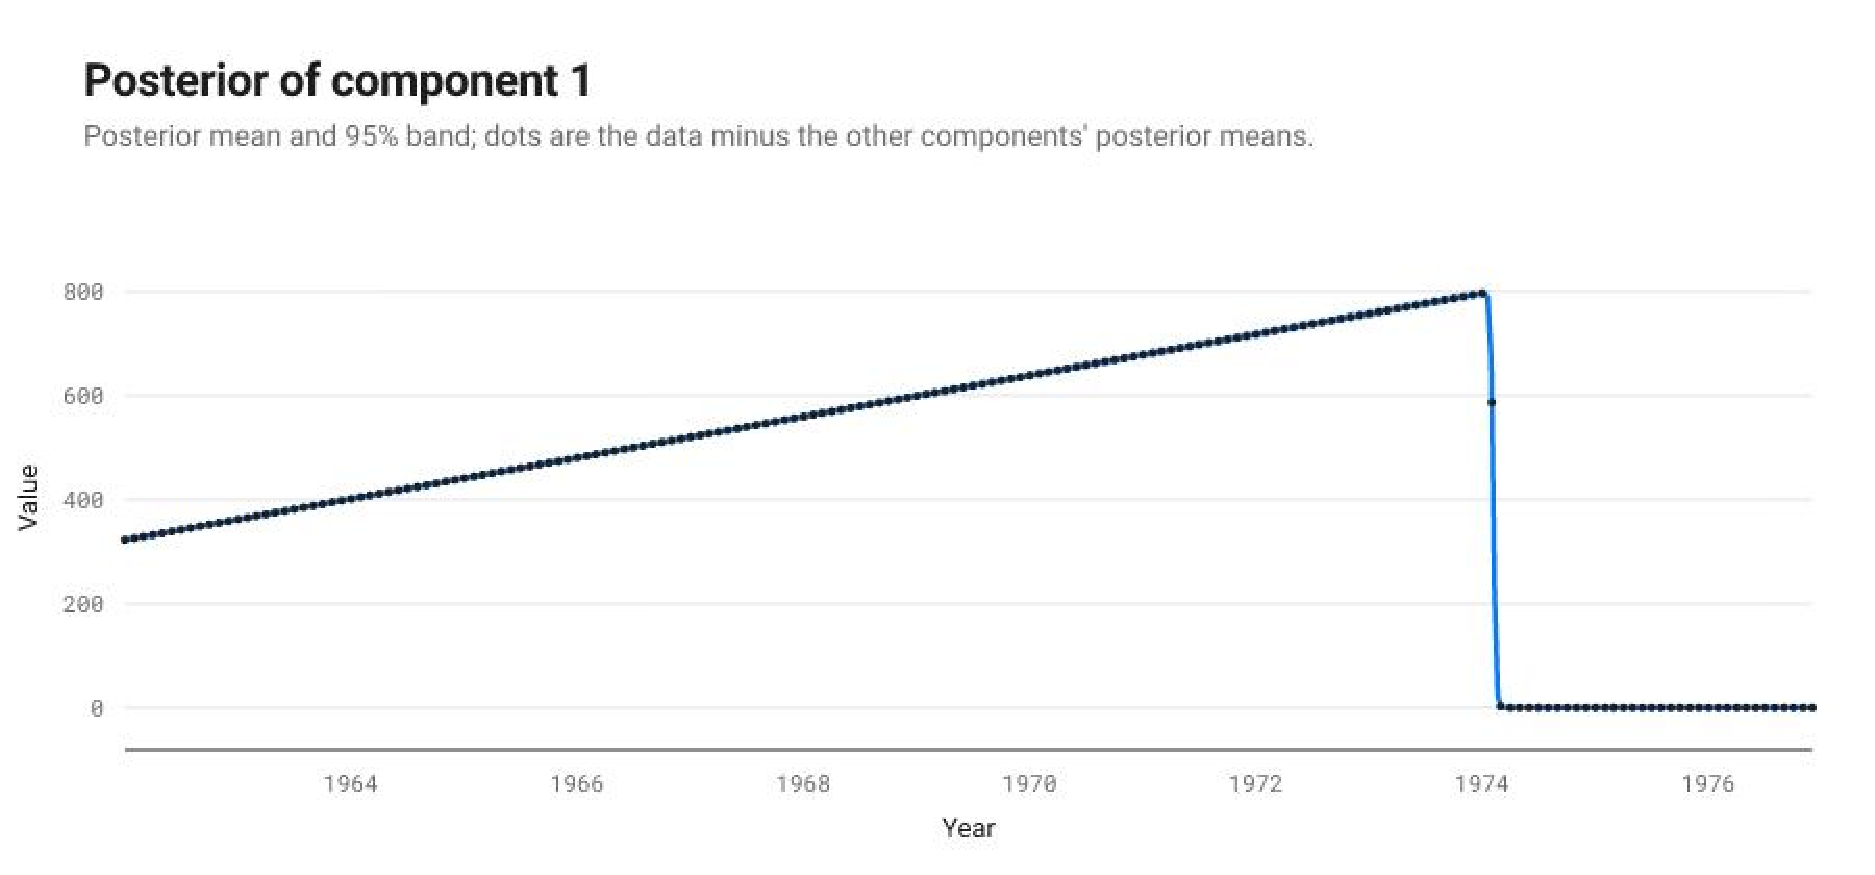
\includegraphics[width=\linewidth]{component_1.pdf}
\caption*{Component 1}
\end{figure}
\subsection*{Component 2: A very smooth monotonically increasing function. This function applies from Feb 1974 onwards}

This component is a very smooth and monotonically increasing function. This component applies from Feb 1974 onwards.

This component explains -78.3\% of the data's variance on its own; with the components above it, 94.5\%. Adding it changes the cross-validated MAE by -51.9\%.

\emph{Extrapolation.} This component is assumed to continue very smoothly but is also assumed to be stationary so its distribution will eventually return to the prior. The prior distribution places mass on smooth functions with a marginal mean of zero and a typical lengthscale of 8.5 years.

\begin{figure}[H]
\centering
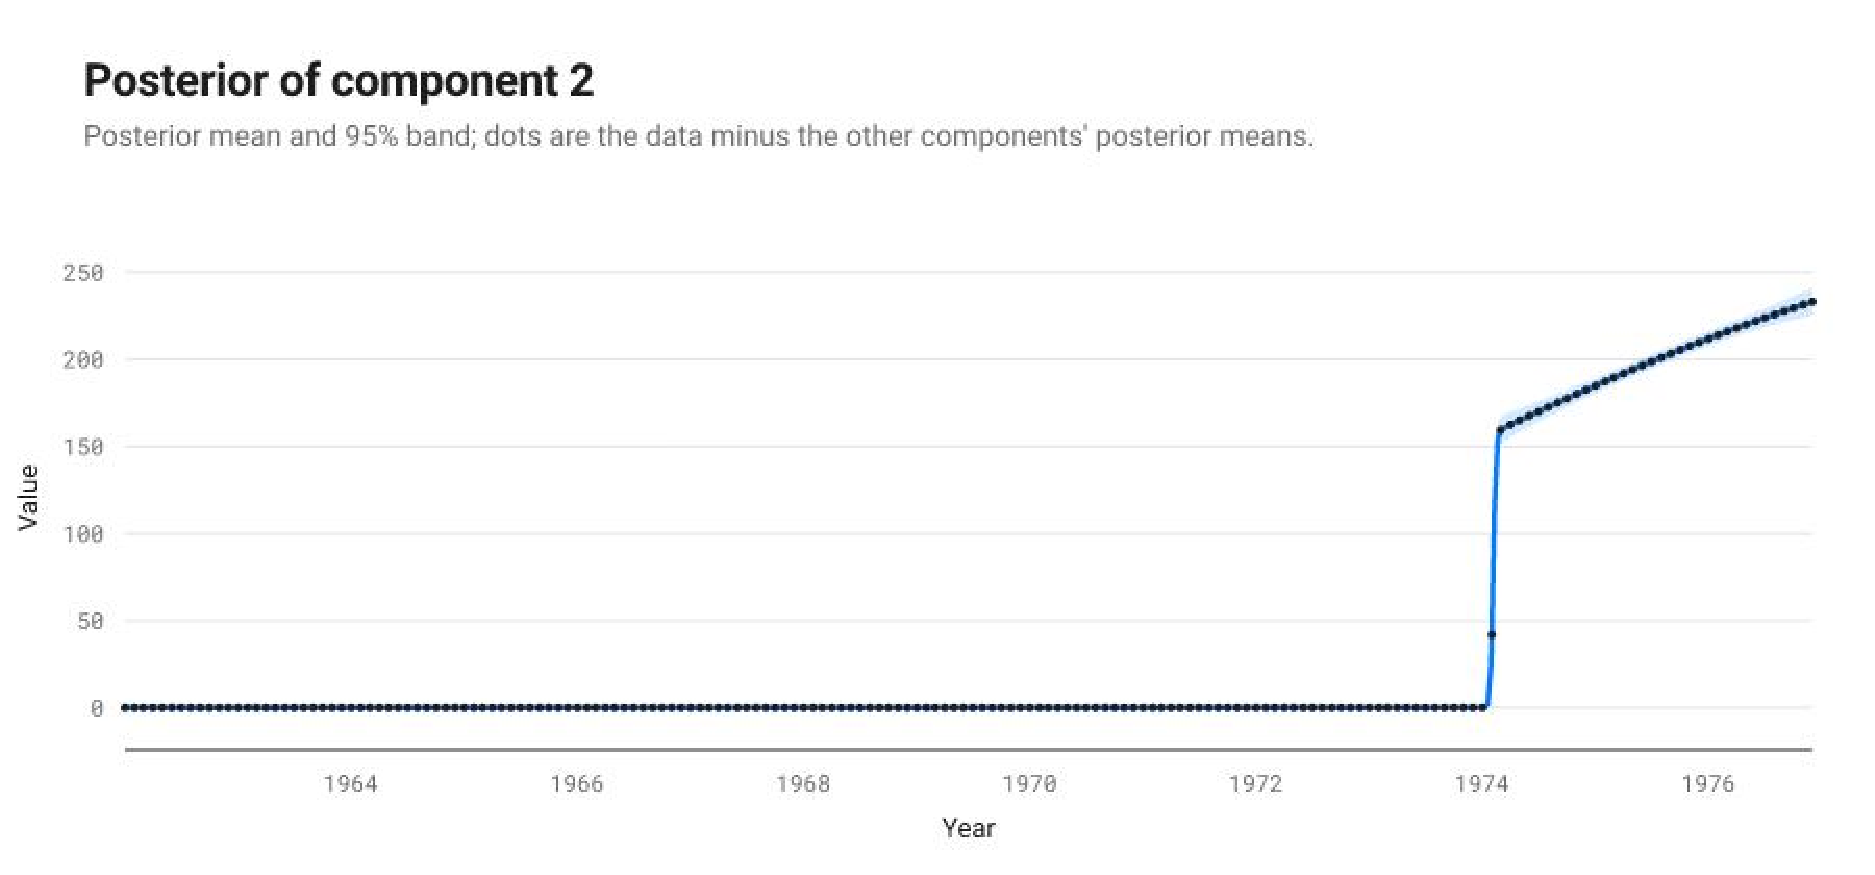
\includegraphics[width=\linewidth]{component_2.pdf}
\caption*{Component 2}
\end{figure}
\subsection*{Component 3: A smooth function with marginal standard deviation increasing linearly away from Feb 1964. This function applies until Feb 1974}

This component is a smooth function with a typical lengthscale of 3.5 months. The marginal standard deviation of the function increases linearly away from Feb 1964. This component applies until Feb 1974.

This component explains 0.0\% of the data's variance on its own; with the components above it, 99.1\%. Adding it changes the cross-validated MAE by -24.1\%.

\emph{Extrapolation.} This component is assumed to stop before the end of the data and will therefore be extrapolated as zero.

\begin{figure}[H]
\centering
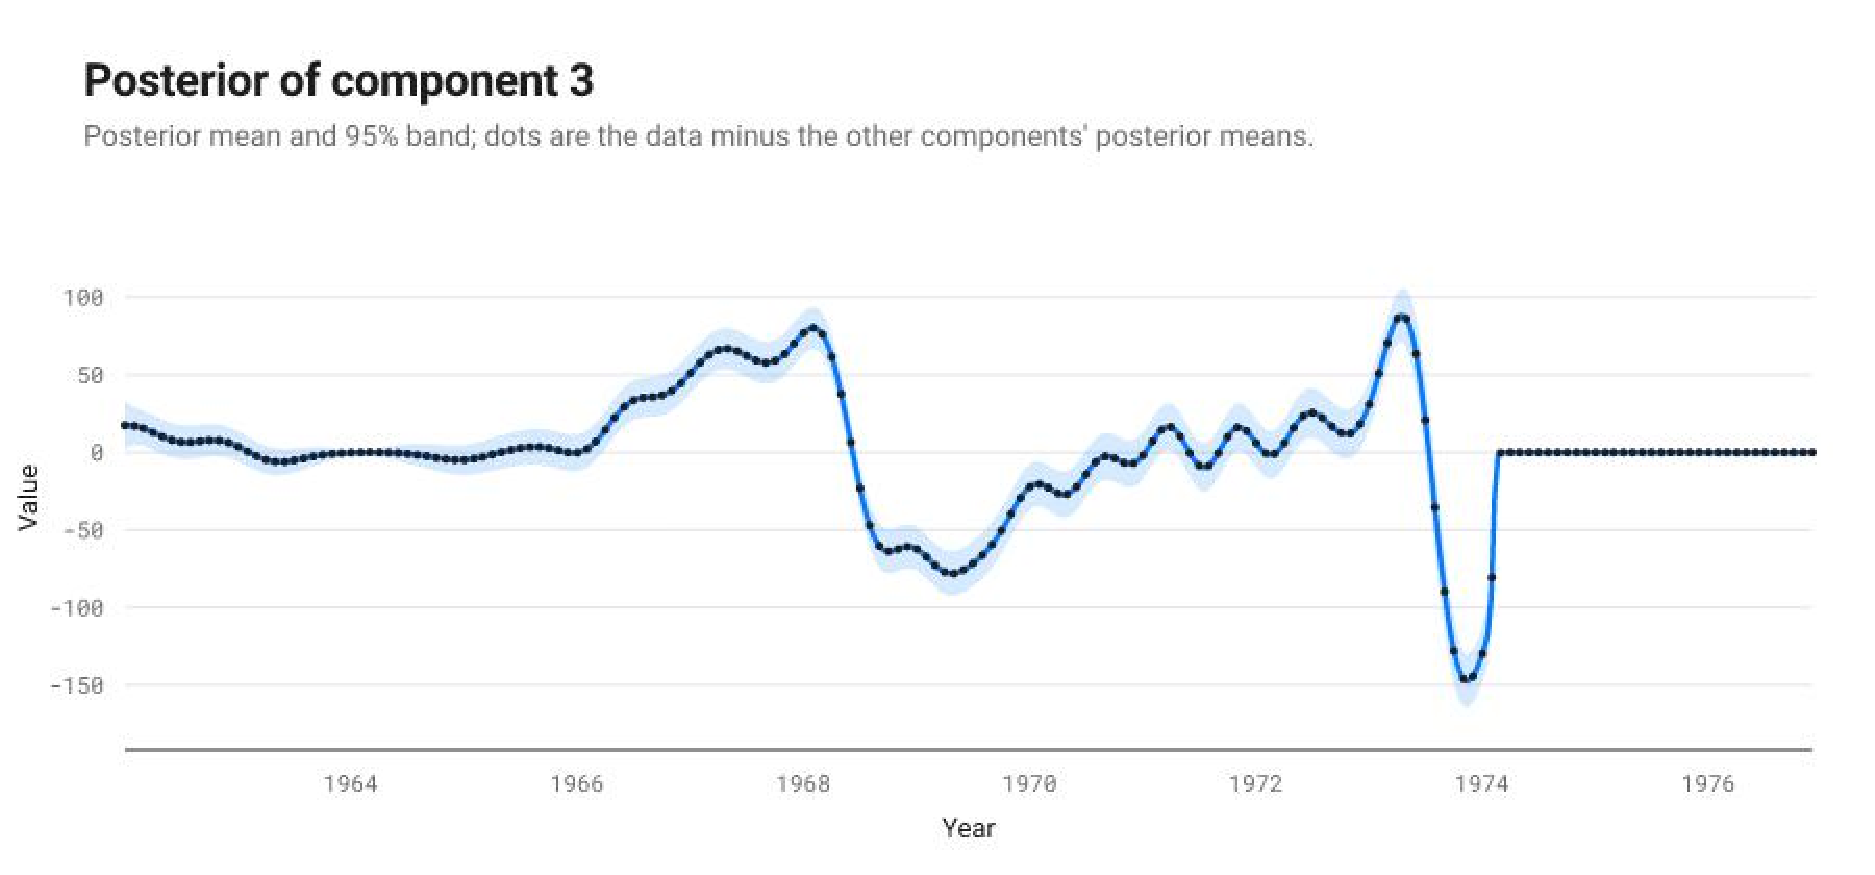
\includegraphics[width=\linewidth]{component_3.pdf}
\caption*{Component 3}
\end{figure}
\subsection*{Component 4: A periodic function with a period of 1.0 years. This function applies until Feb 1974}

This component is periodic with a period of 1.0 years. The shape of this function within each period has a typical lengthscale of 3.9 weeks. This component applies until Feb 1974.

This component explains 0.7\% of the data's variance on its own; with the components above it, 99.7\%. Adding it changes the cross-validated MAE by -13.4\%.

\emph{Extrapolation.} This component is assumed to stop before the end of the data and will therefore be extrapolated as zero.

\begin{figure}[H]
\centering
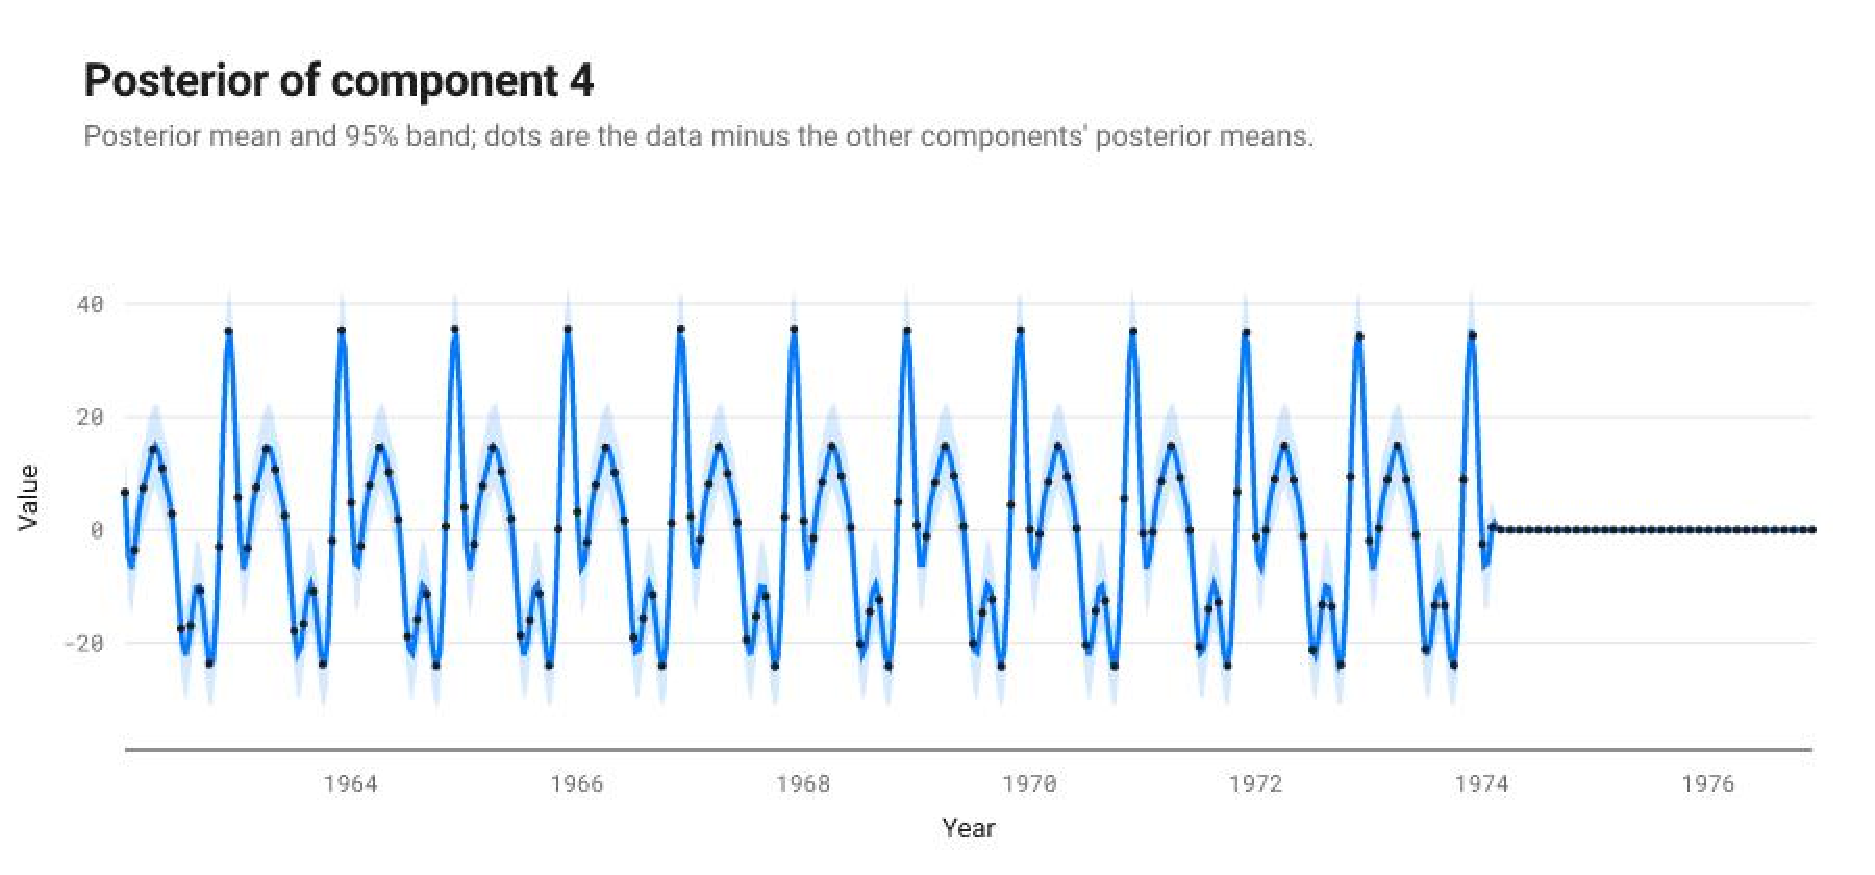
\includegraphics[width=\linewidth]{component_4.pdf}
\caption*{Component 4}
\end{figure}
\subsection*{Component 5: Uncorrelated noise. This function applies until May 1973 and from Oct 1973 onwards}

This component models uncorrelated noise. This component applies until May 1973 and from Oct 1973 onwards.

This component explains 0.4\% of the data's variance on its own; with the components above it, 99.9\%. Adding it changes the cross-validated MAE by -0.0\%.

\emph{Extrapolation.} This component assumes the uncorrelated noise will continue indefinitely.

\begin{figure}[H]
\centering
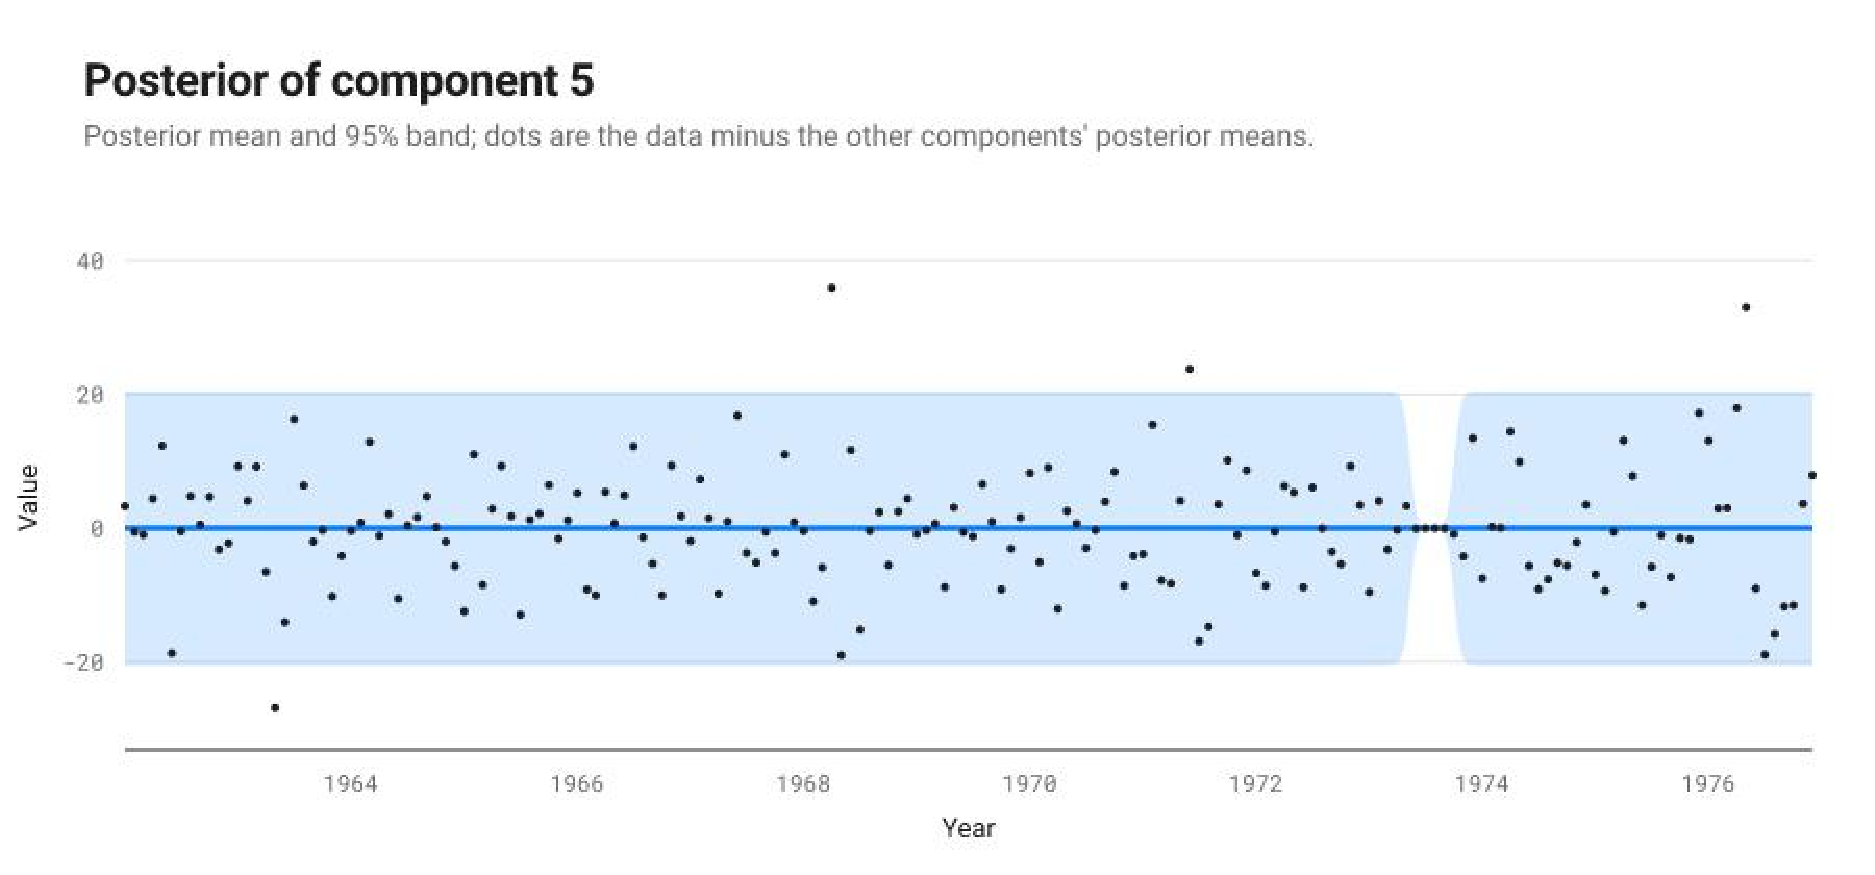
\includegraphics[width=\linewidth]{component_5.pdf}
\caption*{Component 5}
\end{figure}
\subsection*{Component 6: Uncorrelated noise. This function applies from May 1973 until Oct 1973}

This component models uncorrelated noise. This component applies from May 1973 until Oct 1973.

This component explains 0.1\% of the data's variance on its own; with the components above it, 100.0\%. Adding it changes the cross-validated MAE by -0.0\%.

\emph{Extrapolation.} This component is assumed to stop before the end of the data and will therefore be extrapolated as zero.

\begin{figure}[H]
\centering
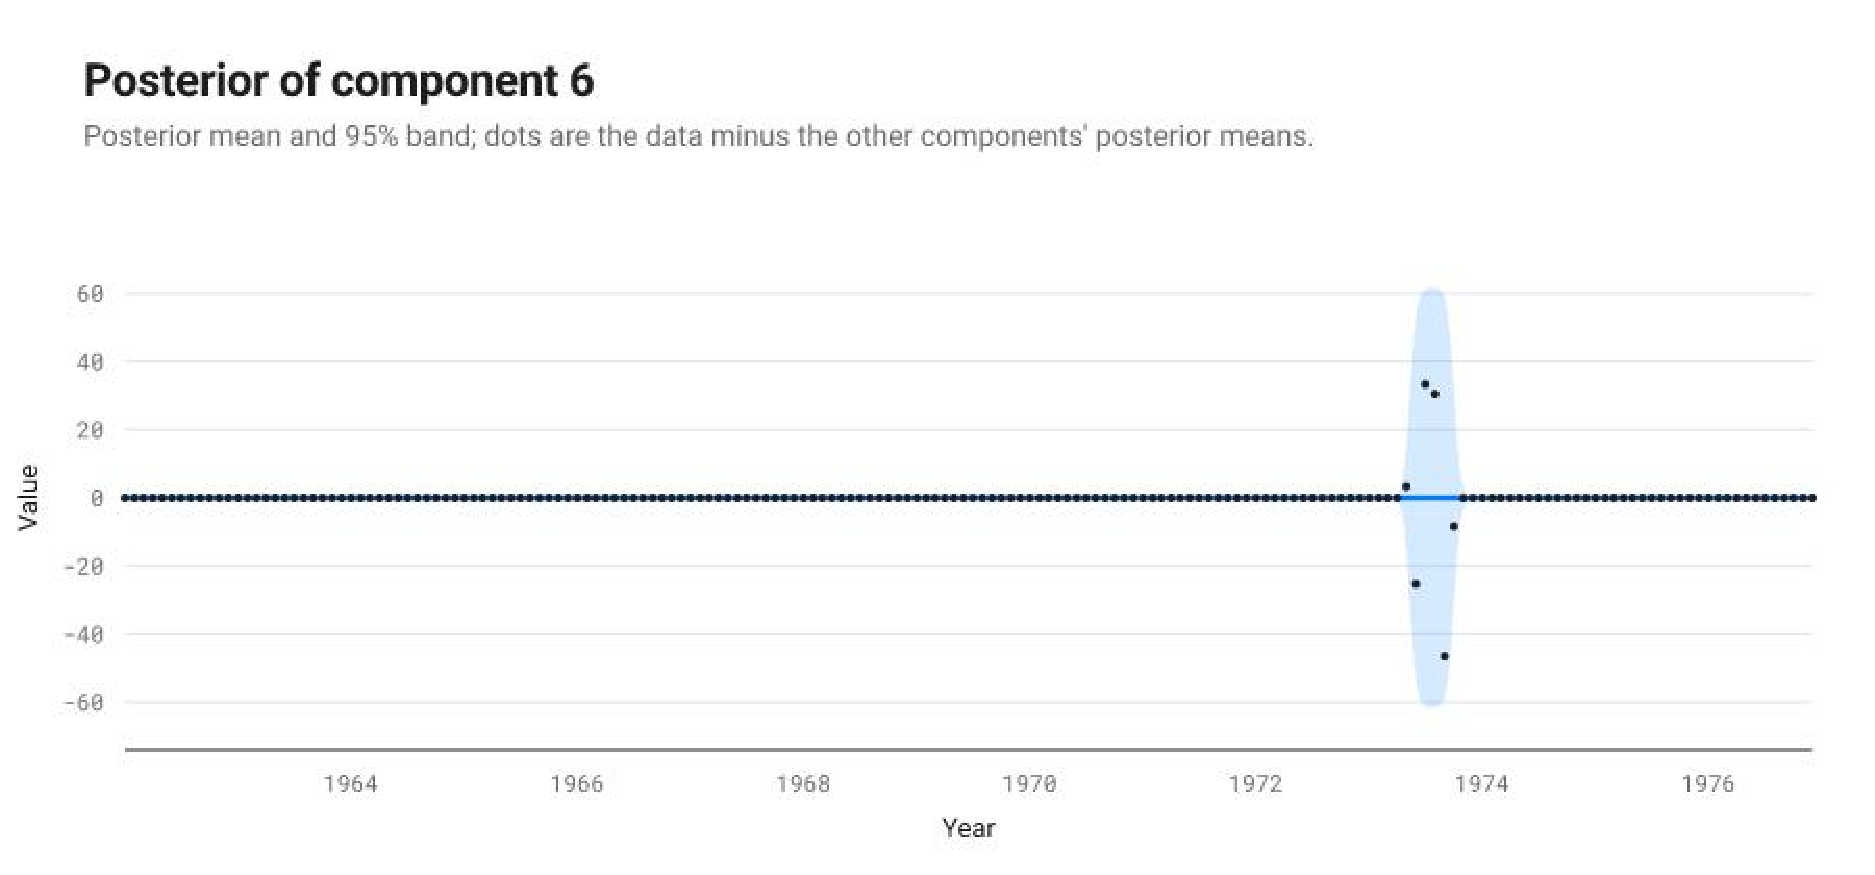
\includegraphics[width=\linewidth]{component_6.pdf}
\caption*{Component 6}
\end{figure}

\section*{Model checking}

Each statistic compares draws of a component's posterior with draws of its prior. A small p-value (bold below 0.05) points at a property of the data that the component's prior does not reproduce.

\begin{center}
\begin{tabular}{lrrrrrrr}
\toprule
\# & QQ max & QQ min & ACF min & ACF min lag & Pgram max & Pgram peak & MMD \\
\midrule
1 & 0.432 & 0.324 & 0.996 & 0.988 & 0.614 & 0.980 & \textbf{0.000} \\
2 & 0.490 & 0.374 & 0.788 & 0.946 & 0.742 & 0.962 & \textbf{0.000} \\
3 & 0.370 & 0.596 & 0.420 & 0.998 & 0.866 & 0.742 & \textbf{0.000} \\
4 & 0.962 & 0.232 & 0.372 & 0.932 & 0.752 & 0.680 & \textbf{0.000} \\
5 & 0.120 & 0.936 & 0.964 & 0.956 & 1.000 & 0.966 & \textbf{0.009} \\
6 & 0.790 & 0.540 & 0.962 & 0.930 & 0.976 & 0.962 & 0.270 \\
\bottomrule
\end{tabular}
\end{center}

QQ: quantile-quantile gaps. ACF: autocorrelation function. Pgram: periodogram. MMD: maximum mean discrepancy two-sample test.

\end{document}
